\chapter{被子植物的功能组织}\label{ch:b1:flowering-plant-organization}

一棵树龄两个世纪的橡树，仍立于它萌发时
所在的那一平方米土地上。它从未进食、从未移动，也从未维持过体温；
然而它已长出四十吨木材，每年夏天都把
五百平方米的叶片伸向空中，并把面积更大的
根表面伸入土壤。被子植物是对
\cref{ch:b1:organism-environment}所提出问题的另一种回答：一株固着的\omterm{def:b1:organism-environment:trophy}{自养}生物，
它应对\omterm{def:b1:organism-environment:organism}{环境}的方式不是把交换过程内化，而是
向外不断生长出交换表面，哪里有光和水，就在哪里生长。
本章讨论这样一种植物体如何组织——其
\omterm{def:b1:mammal-organization:organ}{器官}、组织、所铺展的各类表面，以及构建它们的
生长过程。

\begin{omfigure}
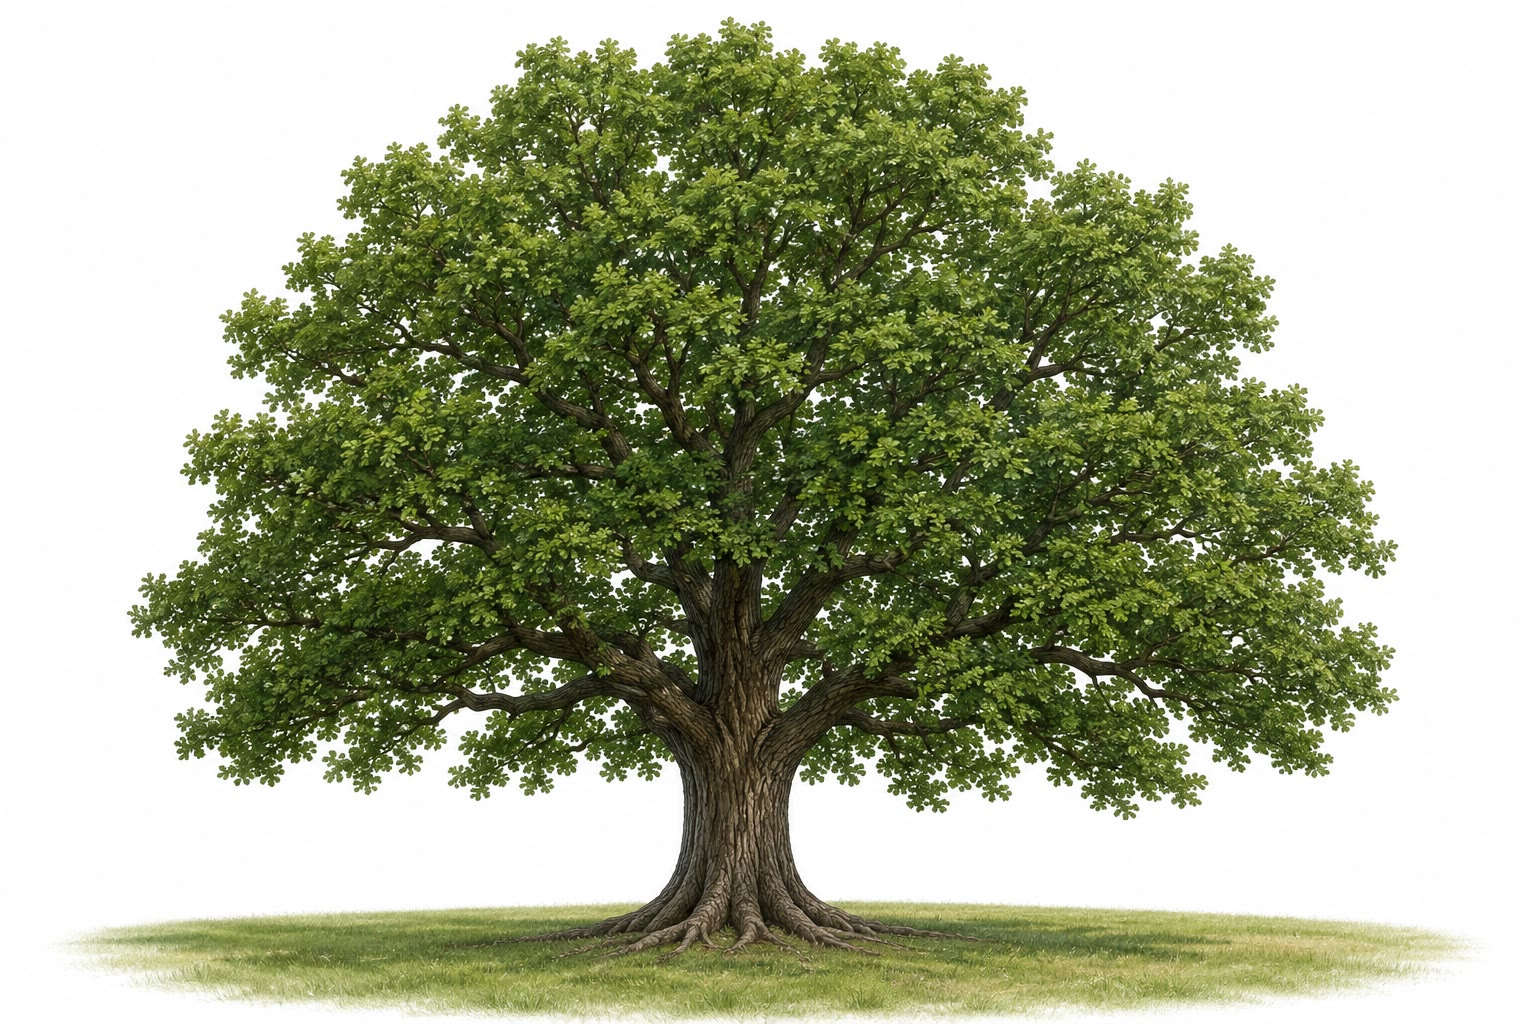
\includegraphics[width=0.62\linewidth]{images/book3/ai/b3-03-oak-tree.jpg}

{\small 夏季里的一棵孤立橡树。其树冠是由叶片组成的阵列，
叶片铺展开以截获光照；草层以下的根系与树冠一样宽，
而其表面积要大数倍。}
\end{omfigure}

\section{营养体}

\begin{definition}[根、茎、叶]\label{def:b1:flowering-plant-organization:organs}
被子植物的营养体由三类
\omterm{def:b1:mammal-organization:organ}{器官}构成。\emph{根}\index{根}固定植株，并吸收
土壤中的水分和矿质离子；它从根尖生长，
并分枝，在根尖后方紧邻处长出\emph{根毛}\index{根毛}。\emph{茎}\index{茎}
把叶片托向光照，并
在根与叶之间输导物质；茎由重复的单元构成，每个单元是
一个带叶和腋芽的\emph{节}\index{节}，以及
位于两节之间的\emph{节间}\index{节间}。
\emph{叶}\index{叶}是光合作用的\omterm{def:b1:mammal-organization:organ}{器官}：一片
表面积大、厚度小的扁平叶片，由叶柄着生于茎上。根构成
根系；茎和叶构成茎叶系统。
\end{definition}

\begin{proposition}[模块化的开放式植物体]\label{prop:b1:flowering-plant-organization:modular}
植物体是\emph{模块化}\index{模块化生长}的：茎是由一系列
相同的单元（节、叶、芽和\omterm{def:b1:flowering-plant-organization:organs}{节间}）依次由顶芽添加而成，
而每个腋芽都可以开始一条新的单元序列。
生长是\emph{无限生长的}\index{无限生长}：没有固定的
成体大小，植物体只要存活，就会不断添加模块，
并由此增加表面积。模块的数目与位置取决于
生境——光照、水分、损伤——因此同一物种在不同地点会呈现
不同形态。哺乳动物的身体则与之相反，是封闭的：
\omterm{def:b1:mammal-organization:organ}{器官}数目固定，体型达到一定大小后即停止生长。
\end{proposition}

\begin{omfigure}
\begin{tikzpicture}[font=\small, >=Stealth, line cap=round]
  % stem axis
  \draw[very thick, omExo!70!black] (0,0) -- (0,6.2);
  \node[circle, fill=omExo!70!black, inner sep=2.2pt] at (0,6.2) {};
  \node[right, font=\footnotesize, align=left] at (0.25,6.35) {顶芽：向上增加 \\ 新模块};
  % nodes with leaves and axillary buds
  \foreach \y/\side in {1.2/1, 2.6/-1, 4.0/1, 5.2/-1} {
    \fill[omExo!70!black] (0,\y) circle (2pt);
    \draw[thick, omExo!70!black] (0,\y) -- (\side*0.6,\y+0.25);
    \draw[thick, omExo, fill=omExo!30] (\side*0.6,\y+0.25) .. controls (\side*1.4,\y+0.6) and (\side*2.2,\y+0.15) .. (\side*2.0,\y-0.1) .. controls (\side*1.4,\y-0.25) and (\side*0.9,\y-0.05) .. (\side*0.6,\y+0.25);
    \fill[omProp] (\side*0.18,\y+0.28) circle (2pt);
  }
  % module bracket
  \draw[thick, gray] (-2.4,1.2) -- (-2.6,1.2) -- (-2.6,2.6) -- (-2.4,2.6);
  \node[left, font=\footnotesize, align=right, gray] at (-2.65,1.9) {一个模块：\\ 节间、节、\\ 叶、腋芽};
  \node[right, font=\footnotesize] at (2.2,4.1) {叶};
  \node[right, font=\footnotesize, omProp] at (0.25,2.95) {腋芽};
  \node[left, font=\footnotesize] at (-0.3,3.3) {节间};
  \node[left, font=\footnotesize] at (-0.3,3.98) {节};
  % roots
  \draw[very thick, omDef!70!black] (0,0) -- (0,-1.6);
  \draw[thick, omDef!70!black] (0,-0.5) -- (-1.0,-1.3) (0,-0.9) -- (0.9,-1.5) (0,-1.2) -- (-0.5,-2.0);
  \foreach \x in {-0.12,-0.06,0.06,0.12} \draw[omDef!70!black] (\x,-1.55) -- (\x*3,-1.9);
  \node[right, font=\footnotesize, align=left] at (0.5,-0.75) {根系：从根尖生长，\\ 根毛位于根尖后方};
  \draw[dashed, gray] (-3.0,0) -- (3.2,0);
  \node[font=\footnotesize, gray, anchor=south east] at (3.2,0.02) {土壤表面};
\end{tikzpicture}

{\small 茎是由模块堆叠而成的结构。每个节带有一片叶和
一个腋芽；顶芽向上添加模块，任一腋芽都可以
开出一个分枝。根系从根尖生长。}
\end{omfigure}

\section{初生植物体的组织}

\begin{definition}[表皮组织系统、基本组织与维管组织]\label{def:b1:flowering-plant-organization:tissues}
植物的每个\omterm{def:b1:mammal-organization:organ}{器官}都由三类组织系统构成。
\emph{表皮组织系统}\index{表皮组织系统}是
\emph{表皮}\index{表皮}，覆盖在\omterm{def:b1:mammal-organization:organ}{器官}表面的单层细胞，
在空气中的部分覆有蜡质的\emph{角质层}\index{角质层}，并
散布有\emph{气孔}\index{气孔}，在根上则由\omterm{def:b1:flowering-plant-organization:organs}{根毛}加以延伸。
\emph{基本组织}\index{基本组织}充满\omterm{def:b1:mammal-organization:organ}{器官}，
包括\emph{薄壁组织}\index{薄壁组织}（活的薄壁细胞，
负责光合作用与贮藏）、\emph{厚角组织}\index{厚角组织}
（活细胞，细胞壁不均匀增厚，是幼茎的柔性支持结构），
以及\emph{厚壁组织}\index{厚壁组织}（细胞壁厚且木质化的细胞，
成熟时已死亡，是刚性支持结构：纤维和
石细胞）。\emph{维管组织}\index{维管组织}负责输导：
\emph{木质部}\index{木质部}向上运输水分和矿质离子，
依靠中空、木质化而死亡的\emph{管胞}\index{管胞}和
\emph{导管}\index{导管}（\cref{ch:b1:plant-transport}）；
\emph{韧皮部}\index{韧皮部}则在活的
\emph{筛管}\index{筛管}中输送糖类，筛管依靠
伴胞维持其活性。
\end{definition}

\begin{omfigure}
\begin{tikzpicture}
  \node[anchor=south west, inner sep=0] (img) at (0,0)
    {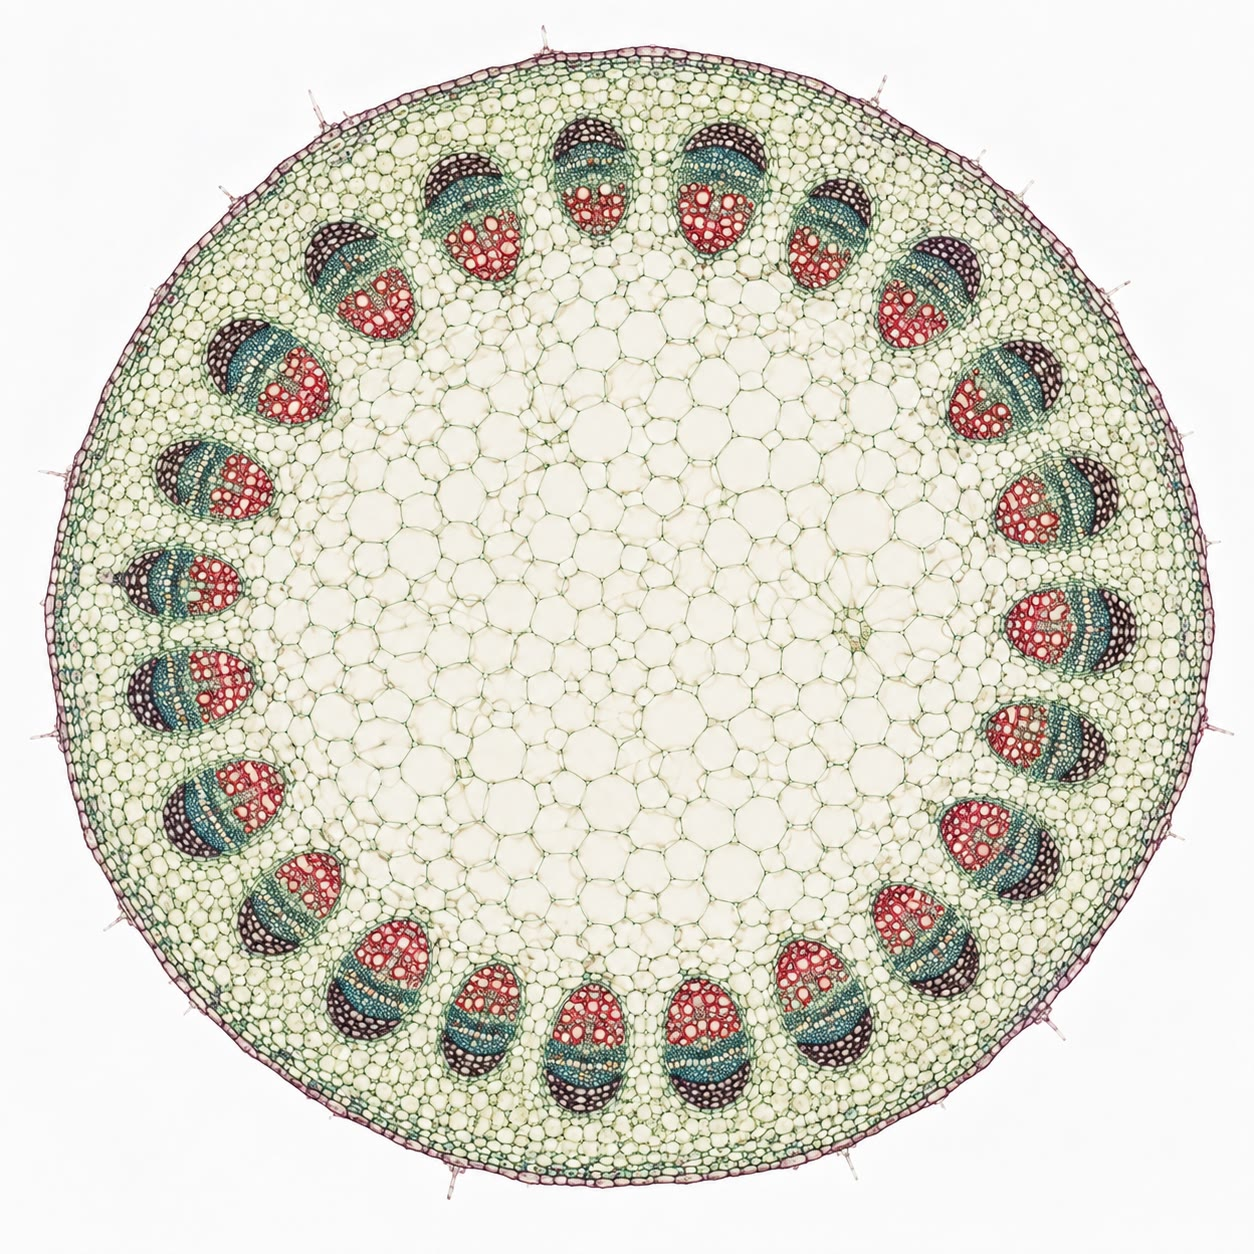
\includegraphics[width=0.5\linewidth]{images/book3/ai/fig-dicot-stem-cross.jpg}};
  \begin{scope}[x={(img.south east)}, y={(img.north west)},
      every node/.style={font=\small}]
    \draw[omDef, thick] (0.50,0.895) -- (0.50,1.06) node[above] {维管束的厚壁组织帽};
    \draw[omDef, thick] (0.87,0.50) -- (1.03,0.60) node[right] {韧皮部（外侧）};
    \draw[omDef, thick] (0.81,0.50) -- (1.03,0.42) node[right] {木质部（内侧）};
    \draw[omDef, thick] (0.50,0.50) -- (-0.03,0.50) node[left] {髓};
    \draw[omDef, thick] (0.085,0.56) -- (-0.03,0.66) node[left] {皮层};
    \draw[omDef, thick] (0.06,0.40) -- (-0.03,0.32) node[left] {表皮};
  \end{scope}
\end{tikzpicture}

{\small 幼嫩双子叶植物茎的横切面。维管束
排列成环：每个维管束中，\omterm{def:b1:flowering-plant-organization:tissues}{木质部}（红染、木质化）朝向
中心，\omterm{def:b1:flowering-plant-organization:tissues}{韧皮部}朝向外侧，外侧有纤维帽覆盖。环内为
髓；环外为皮层和\omterm{def:b1:flowering-plant-organization:tissues}{表皮}。}
\end{omfigure}

\begin{omfigure}
\begin{tikzpicture}
  \node[anchor=south west, inner sep=0] (img) at (0,0)
    {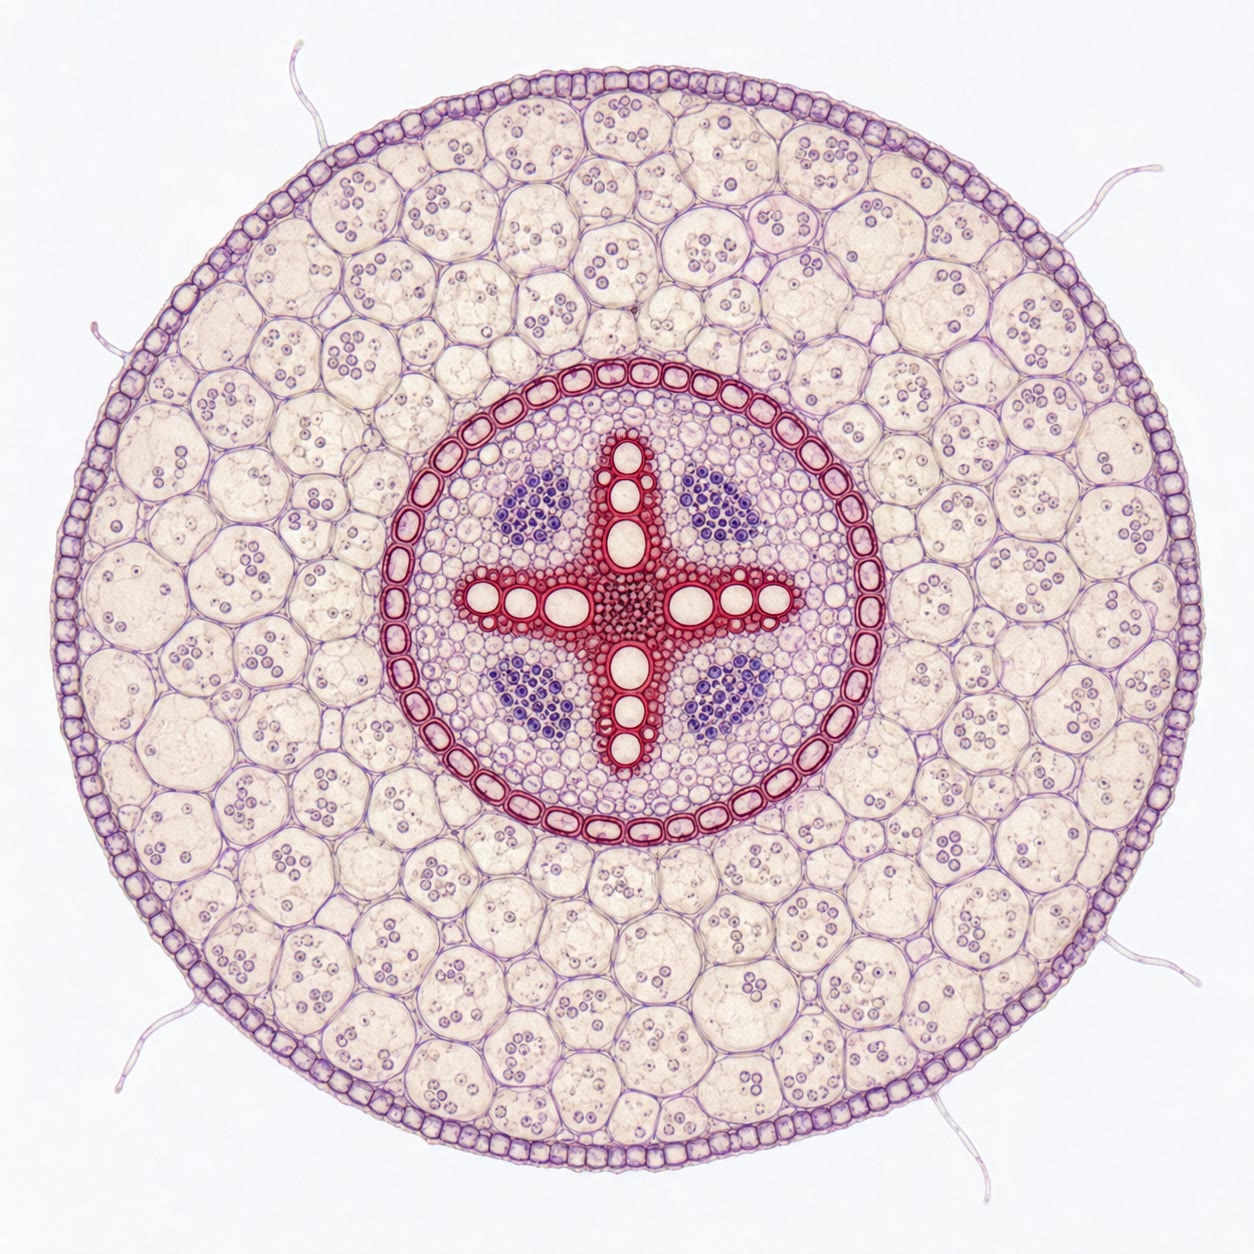
\includegraphics[width=0.46\linewidth]{images/book3/ai/fig-root-cross.jpg}};
  \begin{scope}[x={(img.south east)}, y={(img.north west)},
      every node/.style={font=\small}]
    \draw[omDef, thick] (0.50,0.52) -- (0.50,1.06) node[above] {中央木质部星形};
    \draw[omDef, thick] (0.58,0.45) -- (1.03,0.38) node[right] {韧皮部位于木质部臂之间};
    \draw[omDef, thick] (0.695,0.50) -- (1.03,0.58) node[right] {内皮层};
    \draw[omDef, thick] (0.30,0.50) -- (-0.03,0.50) node[left] {皮层};
    \draw[omDef, thick] (0.06,0.62) -- (-0.03,0.74) node[left] {表皮和根毛};
  \end{scope}
\end{tikzpicture}

{\small 幼嫩双子叶植物根的横切面。中央为单一维管柱：
\omterm{def:b1:flowering-plant-organization:tissues}{木质部}呈星形，\omterm{def:b1:flowering-plant-organization:tissues}{韧皮部}位于星角之间，外界为
\omterm{prop:b1:flowering-plant-organization:stemroot}{内皮层}；其外为较宽的皮层；最外为带有
\omterm{def:b1:flowering-plant-organization:organs}{根毛}的\omterm{def:b1:flowering-plant-organization:tissues}{表皮}。}
\end{omfigure}

\begin{proposition}[茎与根的维管组织排列方式不同]\label{prop:b1:flowering-plant-organization:stemroot}
幼嫩的茎中，\omterm{def:b1:flowering-plant-organization:tissues}{维管组织}形成排列成环的维管束
（双子叶植物），或散布于\omterm{def:b1:flowering-plant-organization:tissues}{基本组织}中（单子叶植物）。每个维管束
\omterm{def:b1:flowering-plant-organization:tissues}{木质部}朝向中心，\omterm{def:b1:flowering-plant-organization:tissues}{韧皮部}朝向外侧；茎中没有
\omterm{prop:b1:flowering-plant-organization:stemroot}{内皮层}，\omterm{def:b1:flowering-plant-organization:tissues}{基本组织}分为中央的髓和
外侧的皮层。幼嫩的根中只有一个中央维管柱：
\omterm{def:b1:flowering-plant-organization:tissues}{木质部}呈星形（双子叶植物为二至五个臂，单子叶植物为多个），
\omterm{def:b1:flowering-plant-organization:tissues}{韧皮部}位于臂之间，维管柱外界为
\emph{内皮层}\index{内皮层}，是一圈细胞，其径向壁
带有防水的带状结构（见\cref{ch:b1:plant-water-minerals}）。这种
排列与功能相适应：茎抵抗弯曲，靠近表面的一圈
维管束使其单位质量最为坚硬；根抵抗
拉伸，中央维管柱正是缆绳的结构。
\end{proposition}

\begin{method}[识别植物切片]\label{met:b1:flowering-plant-organization:section}
\begin{enumerate}
  \item 具有\omterm{prop:b1:flowering-plant-organization:stemroot}{内皮层}的单一中央维管柱：根。
        维管束呈环状或散布，并有髓：茎。扁平的
        \omterm{def:b1:mammal-organization:organ}{器官}，具有两层\omterm{def:b1:flowering-plant-organization:tissues}{表皮}和海绵层：叶。
  \item \omterm{def:b1:flowering-plant-organization:tissues}{木质部}臂较少（2--5）的根为双子叶植物；臂多、环绕髓的为
        单子叶植物。维管束排成一圈的茎为双子叶植物；维管束散布的
        为单子叶植物。
  \item \omterm{def:b1:flowering-plant-organization:tissues}{木质部}可根据其大而壁厚、内部中空的细胞识别，
        （常规染色呈红色）；\omterm{def:b1:flowering-plant-organization:tissues}{韧皮部}为带有\omterm{def:b1:flowering-plant-organization:tissues}{筛管}和伴胞的
        小型活细胞，染色呈绿色或蓝色。
  \item 茎的横切面中，\omterm{def:b1:flowering-plant-organization:tissues}{木质部}朝内，\omterm{def:b1:flowering-plant-organization:tissues}{韧皮部}
        朝外。在根中，\omterm{def:b1:flowering-plant-organization:tissues}{木质部}与\omterm{def:b1:flowering-plant-organization:tissues}{韧皮部}
        沿同一半径交替排列。
\end{enumerate}
\end{method}

\begin{omfigure}
\begin{tikzpicture}
  \node[anchor=south west, inner sep=0] (img) at (0,0)
    {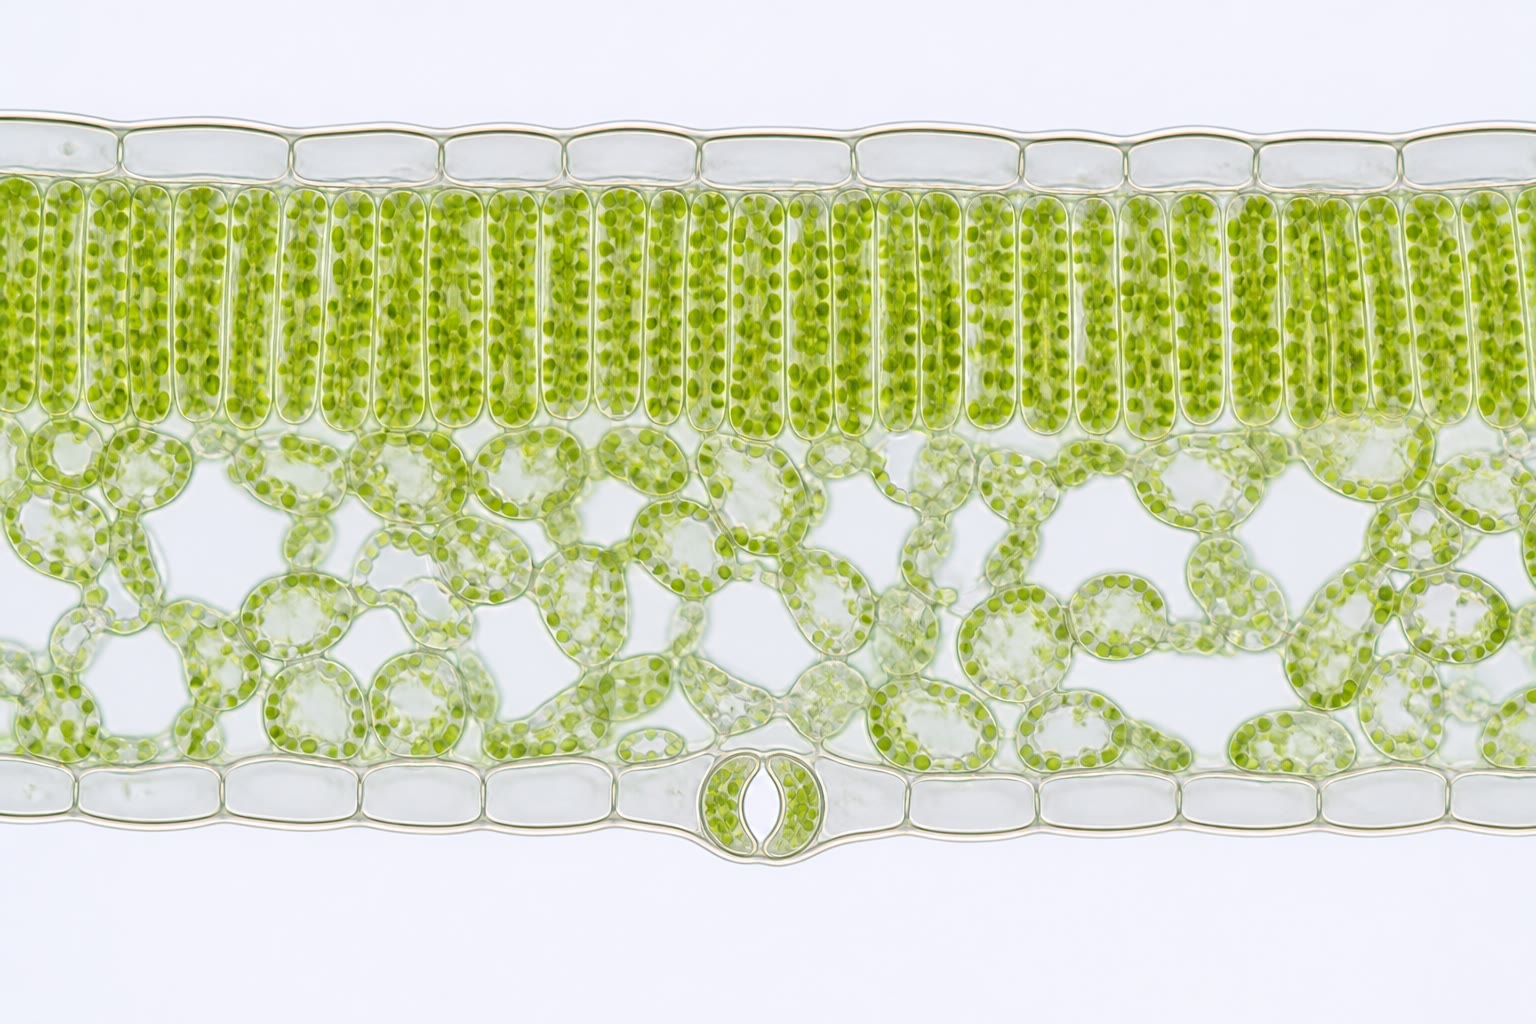
\includegraphics[width=0.48\linewidth]{images/book2/ai/fig-leaf-cross-section.jpg}};
  \begin{scope}[x={(img.south east)}, y={(img.north west)},
      every node/.style={font=\small}]
    \draw[omDef, thick] (0.50,0.94) -- (0.50,1.08) node[above] {上表皮、角质层};
    \draw[omDef, thick] (0.30,0.70) -- (-0.03,0.80) node[left] {栅栏薄壁组织};
    \draw[omDef, thick] (0.30,0.35) -- (-0.03,0.30) node[left] {海绵薄壁组织};
    \draw[omDef, thick] (0.70,0.50) -- (1.03,0.60) node[right] {叶脉};
    \draw[omDef, thick] (0.60,0.10) -- (1.03,0.10) node[right] {气孔};
  \end{scope}
\end{tikzpicture}

{\small 叶的横切面。两层\omterm{def:b1:flowering-plant-organization:tissues}{表皮}之间，
柱状的栅栏细胞内充满叶绿体，朝向光照，
其下疏松排列的海绵细胞之间留有气室，经
\omterm{def:b1:flowering-plant-organization:tissues}{气孔}与外界相通。叶脉输入水分，输出糖类。}
\end{omfigure}

\begin{example}[物质交换发生的场所]\label{ex:b1:flowering-plant-organization:where}
二氧化碳经\omterm{def:b1:flowering-plant-organization:tissues}{气孔}进入叶片，穿过
海绵层的气室，溶解于栅栏细胞湿润的细胞壁中；
栅栏细胞；水分经叶脉的\omterm{def:b1:flowering-plant-organization:tissues}{木质部}到达叶片，
以蒸气形式经同一\omterm{def:b1:flowering-plant-organization:tissues}{气孔}离开。水和离子进入根
经\omterm{def:b1:flowering-plant-organization:organs}{根毛}进入，穿过皮层到达中央的\omterm{def:b1:flowering-plant-organization:tissues}{木质部}。
两种\omterm{def:b1:mammal-organization:organ}{器官}都将交换表面置于外侧，
输导组织则位于中部。
\end{example}

\section{固着的生活：表面}

\begin{definition}[叶面积指数]\label{def:b1:flowering-plant-organization:lai}
植被的\emph{叶面积指数}\index{叶面积指数} $L$ 是
单位地面面积上的单侧叶面积总和。六月的草地
$L \approx 3$，落叶林约为 \qtyrange{4}{6}{}，
热带雨林可达 \qty{8}{}：数层叶片
叠于每平方米土壤之上。
\end{definition}

\begin{proposition}[冠层对光的截获]\label{prop:b1:flowering-plant-organization:beer}
冠层之下到达地面的入射光比例，
在\omterm{def:b1:flowering-plant-organization:lai}{叶面积指数}为 $L$ 的冠层下，呈指数衰减，
\[
\frac{I(L)}{I_0} = e^{-kL},
\]
消光系数 $k$ 介于 $0.3$（直立叶）与
$0.8$（水平叶）之间，通常取 $0.5$。\omterm{def:b1:flowering-plant-organization:lai}{叶面积指数} $L = 5$ 的冠层
$k = 0.5$ 时，截获 $1 - e^{-2.5} = \qty{92}{\%}$ 的光。
\end{proposition}
\begin{proof}
光线向下穿过冠层时，每一薄层叶面积 $\dd L$
截获到达该层光的比例 $k\,\dd L$，其中 $k$ 为
即单位叶面积所遮蔽的水平面积比例（它与叶片的
取向有关）。由此得 $\dd I = -kI\,\dd L$，其解
即指数函数。
\end{proof}

\begin{omfigure}
\begin{tikzpicture}
\begin{axis}[
  width=0.86\linewidth, height=6.2cm,
  axis x line=bottom, axis y line=left,
  xmin=0, xmax=9, ymin=0, ymax=1.1,
  xlabel={叶面积指数 $L$}, ylabel={到达地面的光的比例},
  xlabel style={font=\small, at={(axis description cs:0.5,-0.12)}, anchor=north},
  ylabel style={font=\small},
  tick label style={font=\small}, xtick={0,2,4,6,8}, ytick={0,0.2,0.4,0.6,0.8,1.0},
  legend style={font=\small, at={(0.97,0.95)}, anchor=north east, draw=none},
  clip=false,
]
\addplot[very thick, omDef, domain=0:9, samples=60] {exp(-0.3*x)};
\addlegendentry{$k = 0.3$（直立叶，禾草）}
\addplot[very thick, omThm, domain=0:9, samples=60] {exp(-0.5*x)};
\addlegendentry{$k = 0.5$（典型阔叶）}
\addplot[very thick, omProp, domain=0:9, samples=60] {exp(-0.8*x)};
\addlegendentry{$k = 0.8$（水平叶）}
\draw[dashed, gray] (axis cs:5,0) -- (axis cs:5,0.082);
\node[font=\scriptsize, anchor=west] at (axis cs:5.3,0.36) {栎树，$L=5$：剩余 \qty{8}{\%}};
\end{axis}
\end{tikzpicture}

{\small 三种叶片取向下，冠层之下的光照随\omterm{def:b1:flowering-plant-organization:lai}{叶面积指数}的变化。
当 $L \approx 6$ 之后，多加一层叶片所获得的光
几乎不再增加，这就是冠层在此处停止生长的原因。}
\end{omfigure}

\begin{proposition}[根的表面积超过叶的表面积]\label{prop:b1:flowering-plant-organization:rootsurface}
一株黑麦在体积为 \qty{0.05}{m^3} 的土壤箱中生长四个月，
土壤中共长出 \qty{620}{km} 的根，表面积为 \qty{240}{m^2}，另有
$\num{1.4e10}$ 根\omterm{def:b1:flowering-plant-organization:organs}{根毛}，表面积再增加 \qty{400}{m^2}，
总表面积约为其叶表面积的数百倍，并以每升土壤
含十千米根的密度分布于土壤中。\omterm{def:b1:flowering-plant-organization:organs}{根毛}为管状结构，
由一个\omterm{def:b1:flowering-plant-organization:tissues}{表皮}细胞向外延伸而成，宽 \qtyrange{5}{20}{\micro m}，
长可达一毫米，是大多数吸收作用发生之处；
\omterm{def:b1:flowering-plant-organization:organs}{根毛}只存活数天，并随根尖推进而不断更新。
\end{proposition}
\begin{proof}[证据]
迪特迈尔（1937）将一株黑麦的整个根系从土箱中洗出，
对每一级根的样本以及\omterm{def:b1:flowering-plant-organization:organs}{根毛}
在显微镜下计数和测量，再按比例放大推算：约 1380 万条根，
总长 \qty{623}{km}，另有约 140 亿根\omterm{def:b1:flowering-plant-organization:organs}{根毛}，总长
\qty{10620}{km}。土壤水分和矿物质移动极为缓慢，
根必须位于其一毫米之内才能吸收它们；
根极大的长度，使其能触及每一滴水。
\end{proof}

\begin{omfigure}
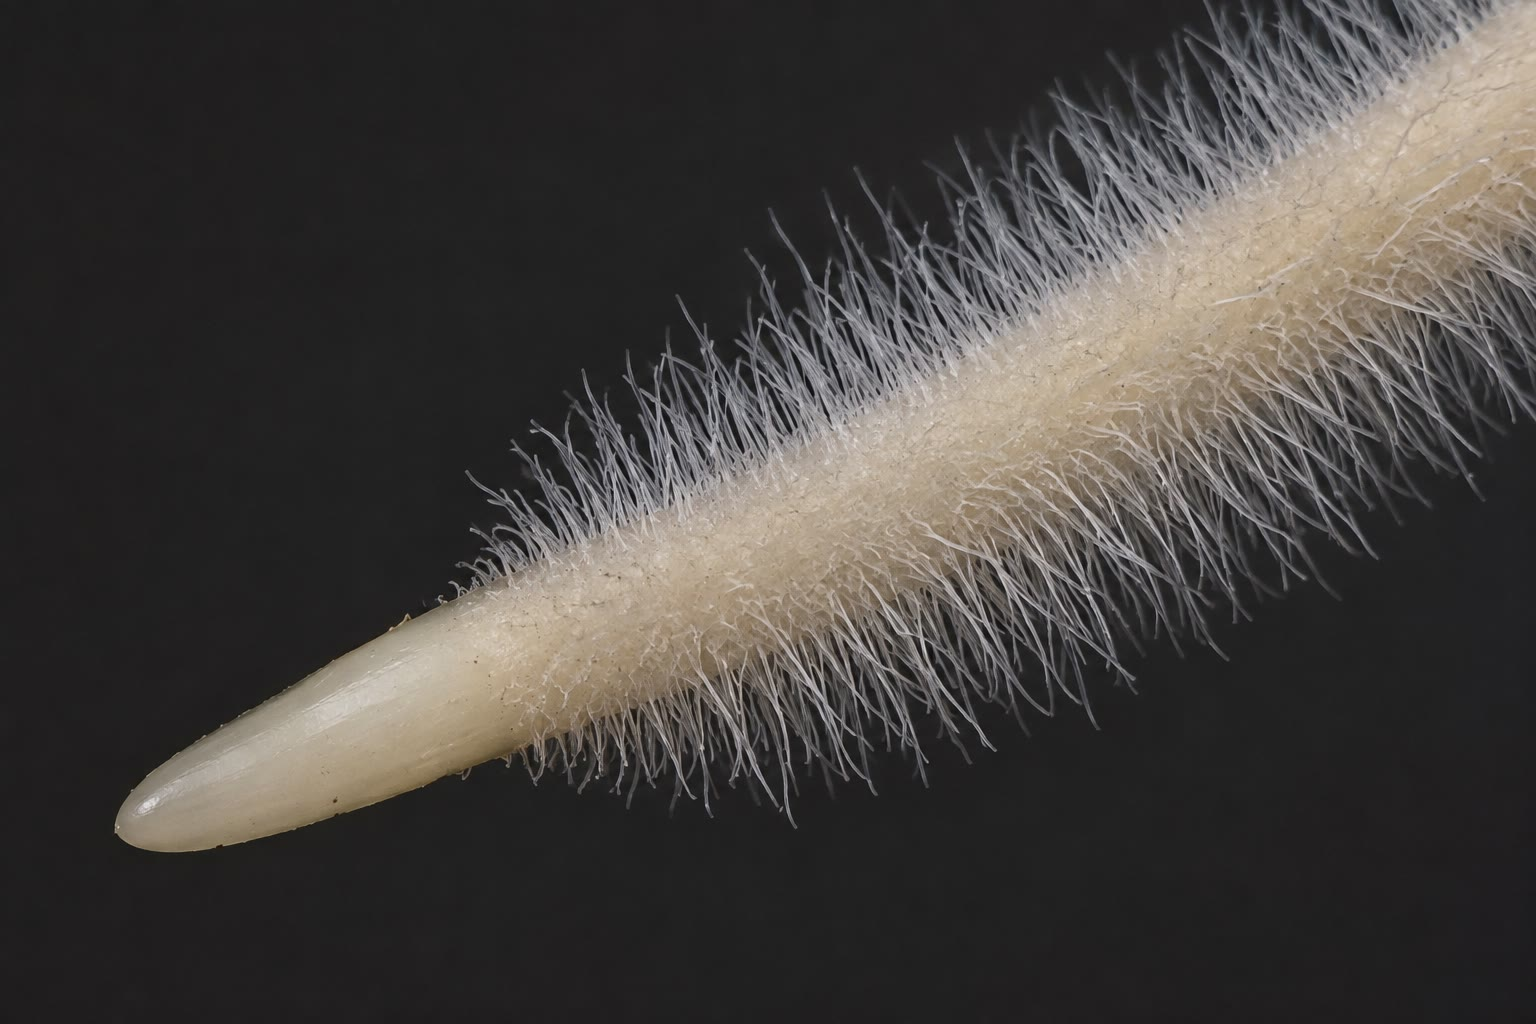
\includegraphics[width=0.58\linewidth]{images/book3/ai/b3-03-root-hairs.jpg}

{\small 萝卜幼苗的\omterm{def:b1:flowering-plant-organization:organs}{根毛}，位于裸露根尖之后数毫米处。
每一\omterm{def:b1:flowering-plant-organization:organs}{根毛}都是伸入土壤的单个\omterm{def:b1:flowering-plant-organization:tissues}{表皮}细胞；
它们共同使吸收表面成倍增加。}
\end{omfigure}

\begin{example}[橡树的两个表面]\label{ex:b1:flowering-plant-organization:oaksurfaces}
一棵橡树的树冠在 $L = 5$ 时遮蔽 \qty{100}{m^2}，并带有
\qty{500}{m^2} 的叶片。其细根约每立方米几千米，穿过 \qty{100}{m^3} 的土壤，
提供数百平方米的表面积，其\omterm{def:b1:flowering-plant-organization:organs}{根毛}再增加约一千平方米：
地下的吸收表面
是地上光合作用表面的数倍，二者覆盖的是
同样面积的地面。
\end{example}

\section{生长与形态}

\begin{definition}[分生组织，初生生长与次生生长]\label{def:b1:flowering-plant-organization:meristem}
\emph{分生组织}\index{分生组织}是由小而未分化的
细胞构成的组织，细胞不断分裂。位于每一茎和根顶端的\emph{顶端分生组织}\index{顶端分生组织}产生\emph{初生
生长}\index{初生生长}：伸长，并形成前述的初生组织。
\emph{侧生分生组织}\index{侧生分生组织}——
\omterm{def:b1:flowering-plant-organization:tissues}{木质部}与\omterm{def:b1:flowering-plant-organization:tissues}{韧皮部}之间的维管形成层，以及\omterm{def:b1:flowering-plant-organization:tissues}{表皮}下的木栓形成层
——产生\emph{次生生长}\index{次生生长}：加粗，向内形成木材（次生\omterm{def:b1:flowering-plant-organization:tissues}{木质部}），向外形成树皮，
见于乔木和灌木的茎与根中。分生组织活动的机制
属于本科二年级分册。
\end{definition}

\begin{omfigure}
\begin{tikzpicture}[font=\small, >=Stealth, line cap=round]
  % root outline (vertical, tip at bottom)
  \draw[thick, omDef!60!black, fill=omDef!8] (-0.7,5.2) -- (-0.7,1.3) .. controls (-0.7,0.4) and (-0.3,0) .. (0,-0.2) .. controls (0.3,0) and (0.7,0.4) .. (0.7,1.3) -- (0.7,5.2);
  % root cap
  \draw[thick, omDef!60!black, fill=omDef!25] (-0.72,0.9) .. controls (-0.75,0.2) and (-0.3,-0.35) .. (0,-0.45) .. controls (0.3,-0.35) and (0.75,0.2) .. (0.72,0.9) .. controls (0.5,0.55) and (0.2,0.4) .. (0,0.45) .. controls (-0.2,0.4) and (-0.5,0.55) .. (-0.72,0.9);
  % meristem
  \fill[omThm!45] (0,0.95) ellipse (0.45 and 0.35);
  % vascular strand
  \draw[thick, omDef!60!black, fill=omDef!30] (-0.15,5.2) -- (-0.15,1.9) .. controls (-0.1,1.5) .. (0,1.35) .. controls (0.1,1.5) .. (0.15,1.9) -- (0.15,5.2);
  % root hairs
  \foreach \y in {3.4,3.7,4.0,4.3,4.6,4.9} { \draw[omDef!60!black] (-0.7,\y) -- (-1.5,\y+0.15); \draw[omDef!60!black] (0.7,\y) -- (1.5,\y+0.15); }
  % zone brackets
  \draw[thick, gray] (2.0,-0.45) -- (2.2,-0.45) -- (2.2,0.6) -- (2.0,0.6); \node[right, align=left, font=\footnotesize] at (2.3,0.1) {根冠：保护根尖，\\ 感受重力};
  \draw[thick, gray] (2.0,0.6) -- (2.2,0.6) -- (2.2,1.4) -- (2.0,1.4); \node[right, align=left, font=\footnotesize] at (2.3,1.0) {分裂区：\\ 顶端分生组织（红色）};
  \draw[thick, gray] (2.0,1.4) -- (2.2,1.4) -- (2.2,3.1) -- (2.0,3.1); \node[right, align=left, font=\footnotesize] at (2.3,2.25) {伸长区：细胞 \\ 伸长至原来的十倍，\\ 推动根尖穿过土壤};
  \draw[thick, gray] (2.0,3.1) -- (2.2,3.1) -- (2.2,5.2) -- (2.0,5.2); \node[right, align=left, font=\footnotesize] at (2.3,4.15) {分化区：\\ 根毛、成熟的木质部 \\ 和韧皮部};
  \node[left, font=\footnotesize, align=right] at (-1.6,4.4) {根毛};
  \node[left, font=\footnotesize, align=right] at (-0.85,2.4) {维管柱 \\ 正在形成};
\end{tikzpicture}

{\small 根尖纵切面。位于保护性根冠之后，
\omterm{def:b1:flowering-plant-organization:meristem}{顶端分生组织}进行分裂，其产物先伸长，再分化
为成熟根的各类组织并长出\omterm{def:b1:flowering-plant-organization:organs}{根毛}。整个
过程仅占数毫米长，随根的
生长而向前移动。}
\end{omfigure}

\begin{proposition}[形态随环境而定]\label{prop:b1:flowering-plant-organization:plasticity}
由于植物的生长是\omterm{prop:b1:flowering-plant-organization:modular}{模块化}且无限的，植物使其
形态与所处\omterm{def:b1:organism-environment:organism}{环境}相适应（\emph{表型可塑性}\index{表型可塑性}）：生长于空旷处的树木枝条低而宽展，同一物种生长于森林中则形成高而无枝的树干；
生长于干旱土壤中的植物会将更多生长投入根系，
处于遮荫之下则更多投入叶片。干旱生境中的物种
（\emph{旱生植物}\index{旱生植物}）具有厚的\omterm{def:b1:flowering-plant-organization:tissues}{角质层}、
藏于凹坑中或由毛保护的\omterm{def:b1:flowering-plant-organization:tissues}{气孔}、小型或多肉的叶片，
以及深扎的根；湿润生境中的物种
（\emph{水生植物}\index{水生植物}）具有薄的\omterm{def:b1:flowering-plant-organization:tissues}{角质层}、位于漂浮叶上表面的\omterm{def:b1:flowering-plant-organization:tissues}{气孔}，
以及充满空气的组织
（\emph{通气组织}\index{通气组织}），将氧气输送至
缺氧淤泥中的根部。
\end{proposition}

\begin{example}[哺乳动物与植物，并列对比]\label{ex:b1:flowering-plant-organization:comparison}
营养：哺乳动物摄取有机物；植物则以
二氧化碳、水和光为原料合成有机物。交换表面：内部的，大小固定，
由血液灌注；外部的，持续生长，由风和
土壤通风。\omterm{def:b1:organism-environment:milieu}{内环境}：温度与成分恒定的受调节体液；
植物则无——细胞自行调节其内容物，植物的
温度取决于空气。生长：达到固定的成体形态；植物则开放、\omterm{prop:b1:flowering-plant-organization:modular}{模块化}，
终生生长。运动：动物走向食物；植物则
朝光和水的方向生长。协调：神经与激素，作用于数秒至数小时之内；
仅靠激素，作用于数小时至数天之内。每一列都是
\omterm{def:b1:organism-environment:organism}{开口系统}的一种自洽存在方式。
\end{example}

\section{练习}

\begin{exercise}[$\star$]\label{exo:b1:flowering-plant-organization:1}
说出开花植物的三种营养\omterm{def:b1:mammal-organization:organ}{器官}，并说明
各自的主要功能。
\end{exercise}

\begin{exercise}[$\star$]\label{exo:b1:flowering-plant-organization:2}
定义枝条的一个模块，并解释
“无限生长”的含义。
\end{exercise}

\begin{exercise}[$\star$]\label{exo:b1:flowering-plant-organization:3}
对每种组织——\omterm{def:b1:flowering-plant-organization:tissues}{表皮}、\omterm{def:b1:flowering-plant-organization:tissues}{薄壁组织}、\omterm{def:b1:flowering-plant-organization:tissues}{厚角组织}、\omterm{def:b1:flowering-plant-organization:tissues}{厚壁组织}，
\omterm{def:b1:flowering-plant-organization:tissues}{木质部}、\omterm{def:b1:flowering-plant-organization:tissues}{韧皮部}——说明其细胞成熟时是否为活的，
以及它的作用。
\end{exercise}

\begin{exercise}[$\star$]\label{exo:b1:flowering-plant-organization:4}
依据光截获图，求到达地面的光所占比例：
在 $L = 3$、$k = 0.3$ 的草地下，以及
在 $L = 6$、$k = 0.5$ 的阔叶林下，各为多少？
\end{exercise}

\begin{exercise}[$\star\star$]\label{exo:b1:flowering-plant-organization:5}
某切片中央为由\omterm{def:b1:flowering-plant-organization:tissues}{木质部}构成的四臂星状结构，臂间为\omterm{def:b1:flowering-plant-organization:tissues}{韧皮部}，
其外为一圈径向壁增厚的细胞环，
再外为一大片圆形细胞区。请判断该\omterm{def:b1:mammal-organization:organ}{器官}与
类群，并分别给出决定各自判断的两个特征。
\end{exercise}

\begin{exercise}[$\star\star$]\label{exo:b1:flowering-plant-organization:6}
借助梁与缆索的力学原理，解释为何
\omterm{def:b1:flowering-plant-organization:tissues}{维管组织}在茎中呈外周环状排列，
在根中则位于中央柱体内。
\end{exercise}

\begin{exercise}[$\star\star$]\label{exo:b1:flowering-plant-organization:7}
某作物的 $L = 4$、$k = 0.6$，其截获的光占多大比例？
若 $L$ 增至 6，截获量将提高多少？
请评论多出的叶片所带来的回报。
\end{exercise}

\begin{exercise}[$\star\star$]\label{exo:b1:flowering-plant-organization:8}
迪特迈尔的黑麦植株有 \qty{623}{km} 的根，
根表面积为 \qty{240}{m^2}。计算根的平均直径。
若其叶片总面积为 \qty{5}{m^2}，
求根加\omterm{def:b1:flowering-plant-organization:organs}{根毛}的表面积与叶片表面积之比。
\end{exercise}

\begin{exercise}[$\star\star$]\label{exo:b1:flowering-plant-organization:9}
\omterm{def:b1:flowering-plant-organization:organs}{根毛}宽 $\qty{10}{\micro m}$、长 $\qty{0.8}{mm}$，
每毫米根上有 \qty{250}{} 根。它们可将
直径为 $\qty{0.4}{mm}$ 的根的表面积放大多少倍？
\end{exercise}

\begin{exercise}[$\star\star\star$]\label{exo:b1:flowering-plant-organization:10}
森林中的一棵树具有 \qty{20}{m} 的光秃树干和一个小树冠；
同一物种生长于田野中时，则自 \qty{2}{m} 处起宽展、多分枝。
请用\omterm{prop:b1:flowering-plant-organization:modular}{模块化}生长以及腋芽在遮荫与光照下的命运，解释这两种形态，
并说明这种可塑性的代价与收益。
\end{exercise}

\begin{exercise}[$\star\star\star$]\label{exo:b1:flowering-plant-organization:11}
\omterm{prop:b1:flowering-plant-organization:plasticity}{旱生植物}的\omterm{def:b1:flowering-plant-organization:tissues}{气孔}藏于覆有毛的凹坑之中。解释
这对叶片气腔与风之间的水汽梯度有何影响，
以及它在二氧化碳吸收上付出了什么代价。为什么
这在沙漠中是划算的，而在雨林中则不利？
\end{exercise}

\begin{exercise}[$\star\star\star$]\label{exo:b1:flowering-plant-organization:12}
“植物没有\omterm{def:b1:organism-environment:milieu}{内环境}。”请用一段文字讨论：植物缺少哺乳动物所具有的哪些东西，
其细胞因此面临什么，
以及植物转而采取的应对方式——表面、生长，以及
它确实进行的调节。
\end{exercise}

\section{问题：一棵橡树的表面}

\begin{problem}[{周末问题——以面积计的橡树叶片、以十亿计的气孔，
以千克计的碳与水，以千米计的根，
最终落在其地面每平方米所铺展的
交换表面上}]
\label{pb:b1:flowering-plant-organization:1}
一棵橡树的树冠遮蔽了 \qty{100}{m^2} 的地面，其\omterm{def:b1:flowering-plant-organization:lai}{叶面积指数}
为 $L = 5$，消光系数为 $k = 0.5$。其叶片下表面
每平方毫米带有 \qty{150}{} 个\omterm{def:b1:flowering-plant-organization:tissues}{气孔}；开放\omterm{def:b1:flowering-plant-organization:tissues}{气孔}的孔隙为
\qty{10}{\micro m} × \qty{5}{\micro m}。在整个冠层上取平均，
并以 \qty{12}{h} 的白昼计，每平方米叶片
每秒吸收 \qty{4}{\micro mol} 的 $\mathrm{CO_2}$，并
散失 \qty{1}{mmol} 的水汽。细根（直径 \qty{0.5}{mm}）
以每立方米 \qty{5}{km} 的密度分布于树冠下方 \qty{1}{m} 深的土层中；
\omterm{def:b1:flowering-plant-organization:organs}{根毛}（\qty{10}{\micro m} × \qty{0.5}{mm}）
每毫米细根上生长 \qty{200}{} 根。摩尔质量：
$\mathrm{CO_2}$ \qty{44}{g/mol}，C \qty{12}{g/mol}，
$\mathrm{H_2O}$ \qty{18}{g/mol}。

\medskip
\noindent\textbf{第一部分——叶与光。}
\begin{enumerate}
  \item 计算树冠的单侧叶面积总和。
  \item 计算到达地面的光的比例，以及
        被截获的光的比例。
  \item 计算橡树仅有 $L = 2$ 时截获的光的比例，
        以及橡树具有 $L = 8$ 时的比例。
  \item 根据这些数值解释为何橡树会停止生长于 $L \approx 5$。
  \item 平均每片叶子的面积为 \qty{50}{cm^2}。
        树冠上共有多少片叶子？
\end{enumerate}

\medskip
\noindent\textbf{第二部分——\omterm{def:b1:flowering-plant-organization:tissues}{气孔}与碳。}
\begin{enumerate}[resume]
  \item 计算树冠上\omterm{def:b1:flowering-plant-organization:tissues}{气孔}的数目。
  \item 计算一个开放\omterm{def:b1:flowering-plant-organization:tissues}{气孔}孔隙的面积，以及开放\omterm{def:b1:flowering-plant-organization:tissues}{气孔}所占
        下表面的比例。
  \item 计算树冠每秒吸收的 $\mathrm{CO_2}$ 量，
        分别以摩尔每秒和克每秒表示。
  \item 计算一个 \qty{12}{h} 白昼中吸收的 $\mathrm{CO_2}$，
        以千克表示，并计算其中所含的碳。
  \item 在一个 \qty{150}{} 天的生长季中，树冠固定了多少碳？
        若一半被树木自身呼吸消耗，
        则它可增加多少质量的木材（含碳 \qty{50}{\%}）？
\end{enumerate}

\medskip
\noindent\textbf{第三部分——水。}
\begin{enumerate}[resume]
  \item 计算树冠每秒散失的水分，
        分别以摩尔每秒和克每秒表示。
  \item 计算每日失水量，以升表示。
  \item 计算失去的水分子数与获得的 $\mathrm{CO_2}$ 分子数之比。
        为何该比值如此之大？
  \item 降雨 \qty{2}{mm} 落在 \qty{100}{m^2} 的地面上，
        若雨水全部到达根部，
        它能供应多少天的蒸腾作用？
\end{enumerate}

\medskip
\noindent\textbf{第四部分——根。}
\begin{enumerate}[resume]
  \item 计算被探索的土壤体积，以及细根的
        总长度。
  \item 计算细根（圆柱体）的表面积。
  \item 计算\omterm{def:b1:flowering-plant-organization:organs}{根毛}的数目。
  \item 计算\omterm{def:b1:flowering-plant-organization:organs}{根毛}的表面积。
  \item 计算地下总吸收表面积，
        及其与单侧叶面积之比。
  \item 细根距离 \qty{1}{mm} 以内的土壤占
        全部土壤体积的比例是多少？（将每条根视为
        半径为 \qty{1}{mm} 的圆柱体的轴。）
  \item 与本章中的黑麦植株相比（\qty{620}{km} 的根位于 \qty{0.05}{m^3} 之中）：
        两者中哪一种植物更充分地探索其土壤，
        且相差多少倍？
  \item 将双侧叶面积与根的表面积相加，
        再除以 \qty{100}{m^2} 的地面面积。
  \item 将此比值与人体的比值相比较，
        即折叠交换表面（\qty{130}{m^2}）与
        外表面（\qty{2}{m^2}）之比。
  \item 用两句话解释，为何植物的该比值在其一生中能不断上升，
        而哺乳动物的该比值却不能。
  \item 给出结果：橡树在其每平方米地面上展开的交换表面
        （地上与地下合计）为多少平方米。
\end{enumerate}
\end{problem}
